\chapter{Decision Trees}\label{ch-dtree}
This chapter is based 
mainly on Ref.\cite{stu-nor-book}.


\begin{figure}[h!]
\centering
\begin{istgame}
\xtdistance{25mm}{50mm}
\istrooto(I){Income?}
\istb{<30K}
\istb{(30K, 100K)}
\istb{100K+}{\text{Loan}}[[draw,fill=green]below]
\endist
\xtdistance{30mm}{30mm}
\istrooto(CR)(I-1){\makecell{Criminal\\Record?}}
\istb{N} 
\istb{Y}{\text{No loan}}[[draw,fill=red]below]
\endist
\istrooto(RD)(CR-1){\makecell{School\\
Teacher?}}
\istb{N}{\text{No loan}}[[draw,fill=red]below]
\istb{Y}{\text{Loan}}[[draw,fill=green]below]
\endist
\istrooto(PL)(I-2){\makecell{Previous\\
loan?}}
\istb{N}
\istb{Y}{\text{Loan}}[[draw,fill=green]below]
\endist
\istrooto(CR2)(PL-1){\makecell{Criminal\\Record?}}
\istb{N}{\text{Loan}}[[draw,fill=green]below]
\istb{Y}{\text{No loan}}[[draw,fill=red]below]
\endist
\end{istgame}
\caption{Example of a decision tree.}
\label{fig-dtree-loan}
\end{figure}


\begin{figure}
\centering
%\setistgameshorten{1.3pt} % use in a TeX group
\begin{istgame}[scale=.7]
\setxtshowarrows{Stealth[open]}(10pt)
\xtShowArrows
\xtdistance{25mm}{50mm}
\istrooto(I){$\rvx_0$}
\istb{p_1}
\istb{p_2}
\istb{p_3}{\rvx_3}[[draw,fill=green]below]
\endist
\xtdistance{30mm}{30mm}
\istrooto(CR)(I-1){$\rvx_1$}
\istb{p_4} 
\istb{p_5}{\rvx_5}[[draw,fill=red]below]
\endist
\istrooto(RD)(CR-1){$\rvx_4$}
\istb{p_8}{\rvx_8}[[draw,fill=red]below]
\istb{p_9}{\rvx_9}[[draw,fill=green]below]
\endist
\istrooto(PL)(I-2){$\rvx_2$}
\istb{p_6}
\istb{p_7}{\rvx_7}[[draw,fill=green]below]
\endist
\istrooto(CR2)(PL-1){$\rvx_6$}
\istb{p_{10}}{\rvx_{10}}[[draw,fill=green]below]
\istb{p_{11}}{\rvx_{11}}[[draw,fill=red]below]
\endist
\end{istgame}
\caption{LD (Linear Deterministic) bnet corresponding to Decision Tree in
Fig.\ref{fig-dtree-loan}. The $p_i$ are
probabilities. The probabilities exiting 
each node
sum to 1.}
\end{figure}


Fig.\ref{fig-dtree-loan}
shows a typical {\bf decision tree (dtree)}.
As you can see,
a dtree contains two main types
of nodes: the non-leaf nodes,
and the leaf nodes.
The {\bf non-leaf nodes} pose
{\bf questions}. In general,
the {\bf answers}\footnote
{The {\bf question-answer pairs}
in dtrees are
also called
{\bf attribute-value pairs}.
Attributes are also
called {\bf features}.}
 to those
questions can
be multiple choices with
two or more choices.
For each of those choices,
a tree branch labeled by the choice
 comes down from the 
question node.
The {\bf leaf nodes} represent
endpoints, goals, final
conclusions, payoffs, etc.
Dtrees can be viewed
as classifiers. They
take in a large amount 
of information about a population 
and compress that information
to just a few classes.
If $S_\rvc$ is the 
set of distinct leaf node labels,
then we call each
$c\in S_\rvc$
a  {\bf class of the classifier}.
In the case of
Fig.\ref{fig-dtree-loan},
$S_\rvc=\{\text{No Loan, Loan}\}$.

Dtrees can be used 
with
probabilities attached to each node, or without
probabilities
(as a
plain undirected graph(UG)).
This is analogous to bnets,
which can be used with
probabilities attached to each node
 (as DAGs with
TPMs specified for each node) or without
probabilities (as plain
DAGs).
Dtrees differ 
from bnets in that
their tree branches 
are labelled, whereas bnet arrows
 aren't labelled.
Also,
whereas the nodes of
a bnet carry a matrix of 
probabilities (the TPM),
the nodes of a dtree carry
just a column vector
of probabilities
which represents
a single 
probability distribution.
Henceforth,
we will refer to
the column vector
of probabilities
carried by each node of a dtree
as its {\bf Transition
Probability Vector (branch probablities)}.
Without the branch probablities,
a dtree can be used 
as a deterministic classifier,
to classify inputs.
With the branch probablities,
it can be used as a 
probabilistic sampler (to generate
random samples.)

A trivial 
observation
that is seldom made
in the dtree pedagogical literature
is that every dtree 
maps into a special bnet, 
let's call it
its \qt{image} bnet,
in a very natural way.
We use the dtree
of Fig.\ref{fig-dtree-loan}
as an example to show 
how to do this. 

can be learned from
a dataset
following
the dtree Structure Learning (SL)
algorithm
discussed in Section \ref{sec-dtree-sl}.



When drawing dtrees,
some people put
info 
like explanations 
and probabilities on the
branches
of  the dtree.
That
info can all
be preserved
in the TPM
and  the
node names and
 node state names
of the image bnet nodes.
One can also place info
inside tool tips attached to
the node name and node state names.
Often,
the pedagogical literature
states that 
dtrees are more explicit and  
carry
more info than their
image bnets,
but if one 
follows the above
prescriptions,
both can carry
the same info.



A naive Bayes (NB) bnet 
(see Chapter \ref{ch-naive})
consists of a single \qt{class node}
with states $S_\rvc$ that fans
out with arrows 
pointing to the
\qt{feature nodes}.
If each leaf node
of a NB bnet
fans out into 
a set of new leaf
nodes, and those new
leaf nodes
also
fan out
and so on,
we get a 
generalized NB bnet.
Let's call
this type of tree bnet an $NB^*$ bnet.
An $NB^*$ bnet
has the same graph structure
as the image bnet of a dtree,
but it's more general,
because its 
TPMs are more general. 
Each 
TPM of a $NB^*$ bnet
 can have several non-trivial
columns instead of just one
branch probablities= $\vec{p}$.


\section{Structure Learning for  Dtrees}\label{sec-dtree-sl}



Let

$J_0=\{0,1, \ldots, nj-1\}$

$\Sigma=\{0,1,2, \ldots,nsam-1\}$

$DS=\{(\s, x^\s, c^\s): \s\in \Sigma\}$ be a dataset

$\s\in \Sigma$ be an individual (a sample)
from a population, 

$x^\s\in S_\rvx$ be the {\bf
feature (attributes, questions) vector}.
$S_\rvx= S_{\rvx_0}\times S_{\rvx_1}
\times\ldots\times S_{\rvx_{nj-1}}$,
$x=(x_0, x_1, \ldots, x_{nj-1})\in S_\rvx$, 
$x_j\in S_{\rvx_j}$


$c^\s\in S_\rvc$ be a {\bf classification class}

We will
assume $S_\rvx$ and $S_\rvc$ are finite sets.

Building a {\bf classifier $Y$} 
(curve fit) for a dtree means
finding a deterministic
function $Y:S_\rvx\rarrow S_\rvc$ 
such that 
$c^\s \approx Y(x^\s)$
for all $\s\in \Sigma$.
If we divide
the population
$\Sigma$ 
into two large 
disjoint
sets, a {\bf training set} $\Sigma_{train}$
and a {\bf validation set} $\Sigma_{vali}$,
and if $c^\s \approx Y(x^\s)$ very closely
for $\s\in \Sigma_{train}$
but fits poorly
for $\s\in \Sigma_{vali}$,
then we say the classifier  $Y$
suffers from {\bf overfitting}.
We can learn the structure
and TPVs of a dtree from a dataset $DS$,
by using the
dtree {\bf Structure Learning (SL)}
algorithm that we will 
discuss in detail later. However,
that algorithm
is prone to produce
a classifier $Y$ that overfits.
Two techniques 
commonly used to 
reduce the effects of overfitting
are {\bf pruning}  and 
{\bf Random Forest (RF)}
(see Chapter \ref{ch-rforest}).
Pruning just means somehow
removing nodes that are
too specific. 
An RF is an ensemble of dtrees 
that one averages over.
In this chapter, we will only deal
with a single dtree,
not an ensemble of them. 

Dtree SL was invented in 1984-1986 so it
is fairly old.
Many in the AI
community 
consider dtrees old fashioned
compared to neural nets.
But dtrees 
are {\bf interpretable} whereas neural nets aren't.\footnote{
To be precise, only
plain dtrees without boosting or
 bagging
are interpretable.
Dtrees used within boosting
(see Chapter \ref{ch-adaboost} on AdaBoost
and
Chapter \ref{ch-xgboost} on XGBoost)
or bagging
(see Chapter \ref{ch-rforest} on Random Forest)
gain much
accuracy but lose
{\bf interpretability}.}
Bnets are interpretable too.


Below,
we give the standard
algorithm for SL
of a dtree, in the form
of pseudo-code.
But first,
we define
two quantities,
Information Gain and
Gini,
that are 
used in that 
pseudo-code.


\subsection{Information Gain, Gini}
This section uses various Shannon Information Theory
entropies. Our 
notation for those
entropies
is described in Chapter \ref{ch-conventions}.


Call a {\bf separation ability measure} (SAM)
a measure used 
to decide, when 
constructing a dtree from a dataset,
in what order 
to ask the questions
about the feature vector $x$.
The question order is decided
by searching 
over all so far unused questions
for the question with 
the largest SAM.\footnote{SAM
is also called, somewhat
confusingly, the splitting
criterion and Gain.}




Let $N_j(c, x_j)$ is the number
of individuals $\s$
in the population that exits question node $j$,
belonging to class $c$ and having $\rvx_j=x_j$.
From $N_j(c, x_j)$, we can define 
an empirical
probability distribution 

\beq
P_j(c, x_j)
=
\frac{N_j(c, x_j)}{N_j}
\;,\;\; \text{ where }
N_j=\sum_{c, x_j}N_j(c, x_j)
\eeq

Once
we have an empirical probability distribution
$P_j(c, x_j)$ for each node $\rvx_j$,
we can define

\beqa
IG_j
&=&
H_j(\rvc)-H_j(\rvc|\rvx_j)
\\
&=& H_j(\rvc:\rvx_j)
\label{eq-info-gain}
\eeqa
$IG_j$
is called the {\bf
information gain
for node $\rvx_j$}.
Maximizing this mutual information
produces 
a node $\rvx_j$ that has 
a large correlation
to a class $c$.
If the  
goal is to reach
a point 
where each leaf node is
closely correlated
to a different class,
then maximizing the
Information Gain
of each new node
is a greedy move
towards that goal.
Thus, Information Gain
is a good 
SAM
for dtree SL.

If we approximate

\beqa
\ln  P_j(c|x_j)
&\approx&
\ln [1 + P_j(c|x_j)-1]
\\
&\approx&
P_j(c|x_j)-1
\eeqa
in $H_j(\rvc|x_j)$,
we get what is called 
the {\bf Gini (or Gini Index)
for node $\rvx_k$}:


\beqa
H_j(\rvc|x_j)
&=&
-\sum_c P_j(c|x_j)\ln P_j(c|x_j)
\\
&\approx&
1 -\sum_{c\in S_{\rvc}} P_j(c|x_j)^2
\eqdef
 Gini_{x_j}
\eeqa
$Gini_{x_j}$
is a fairly good
polynomial approximation
to $H_j(\rvc|x_j)$.\footnote{
The average of $H(\rvc:b)$ over
$b$ is $H(\rvc:\rvb)=\sum_bP(b)
H(\rvc:b)$.
Likewise,
the average of
$H(\rvc|b)$ over $b$ is 
$H(\rvc|\rvb)=\sum_b P(b)H(\rvc|b)$.
$H(\rvc:\rvb)$ 
becomes $H(\rvc:b)$
and $H(\rvc|\rvb)$
becomes $H(\rvc|b)$
when 
$P(b)$ is a delta function.
}
It is computationally
much less expensive than
$H_j(\rvc|x_j)$,
because it does not
require computing a log.

We say 
a probability 
distribution $P_\rvx$, is {\bf pure (i.e., deterministic)}
 if $P_\rvx(x)=\delta(x, x_0)$. $Gini_{x_j}$
 and $H_j(\rvc|x_j)$ are both always
non-negative.
They both vanish iff  
$P_j(c|x_j)$ is pure.
Thus, $Gini_{x_j}$ and  $H_j(\rvc|x_j)$ 
are both good measures of  {\bf class impurity}.

The {\bf average Gini of node $\rvx_j$} is defined as

\beq
AGini_j
=
\sum_{x_j\in S_{\rvx_j}}
P_j(x_j)
 Gini_{x_j}
\;.
\eeq
It measure 
the average impurity
of the children of node $\rvx_j$.



\begin{mdframed}[hidealllines=true,backgroundcolor=blue!10]
In practice, the
SL algorithm
is done recursively.
Each 
recursion
step 
decides
which feature $x_j$
will be the root 
node of the current tree.
For all \qt{candidate} features
(i.e., all $\rvx_j$
that haven't been used yet 
as tree nodes), one
calculates
$IG_j$,
either
exactly
or approximately via Gini's,
using the following formula:

\beq
IG_j=
H_j(\rvc)
-
\sum_{x_j\in S_{\rvx_j}}
P_j(x_j)
\underbrace{H_j(\rvc|x_j)}_
{\approx Gini_{x_j}}
\eeq
One then chooses $j=\argmax_j IG_j$. This
maximizes the $\rvc-\rvx_j $ correlation.

Alternatively,
some software programs use
the average Gini
$AGini_j$
as their SAM. They
choose
as root node
 $j=\argmin_j AGini_j$.
This minimizes the average impurity
of the children of node $j$.
Since $IG_j$
differs from $AGini_j$ by $H_j(\rvc)$,
maximizing $IG_j$
and
minimizing $AGini_j$
might lead  to different results.
\end{mdframed}
\hrule\noindent{\bf Example of calculation of $AGini_j$ 
and $IG_j$}

Suppose we deduce from a dataset
the numbers in the yellow cells
in Table \ref{tab-temp-gini}.
These numbers are repeated in  Fig.\ref{fig-stump-3cildren}.
Then we can calculate the white cells as follows: 

% Please add the following required packages to your document preamble:
% \usepackage[table,xcdraw]{xcolor}
% If you use beamer only pass "xcolor=table" option, i.e., \documentclass[xcolor=table]{beamer}
\begin{table}[h!]
\centering
\begin{tabular}{|l|l|l|l|}
\hline
$j=temp?$ & \cellcolor[HTML]{CBCEFB}$x_j=hot$ & \cellcolor[HTML]{CBCEFB}$x_j=med$ & \cellcolor[HTML]{CBCEFB}$x_j=cold$ \\ \hline
\rowcolor[HTML]{FFFFC7} 
\cellcolor[HTML]{9AFF99}$c=play$ & 3 & 3 & 3 \\ \hline
\rowcolor[HTML]{FFFFC7} 
\cellcolor[HTML]{FFCCC9}$c=stay$ & 1 & 2 & 2 \\ \hline
$Gini$ & 0.375 & 0.48 & 0.48 \\ \hline
\multicolumn{4}{|l|}{$AGini=0.45$} \\ \hline
$H_j(\rvc|x_j)$ & $\approx 0.375$ & $\approx 0.48$ & $\approx 0.48$ \\ \hline
\multicolumn{4}{|l|}{$IG\approx 0$} \\ \hline
\end{tabular}
\caption{Evaluating AGini and IG for node $temp$.}
\label{tab-temp-gini}
\end{table}



\begin{figure}[h!]
\centering
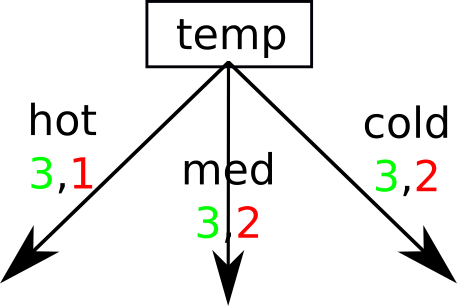
\includegraphics[width=1.5in]
{dtree/stump-3children.png}
\caption{Tree stump
corresponding to Table \ref{tab-temp-gini}.}
\label{fig-stump-3cildren}
\end{figure}



\begin{itemize}
\item Gini(hot)$=1-(3/4)-(1/4)=0.375$
\item Gini(med)$=1-(3/5)^2-(2/5)^2=0.48$
\item Gini(cold)$=1-(3/5)^2-(2/5)^2=0.48$
\item AGini $ = (4/14)(0.375)+
(5/14)(0.48) + (5/14)(0.48) = 0.45 $
\item IG $\approx [1 -(6/9)^2-(3/9)^2]-AGini= 
0.44-0.45\approx 0$
\end{itemize}

This gives
the AGini and IG for just one 
candidate root node.
We would have
to calculate
AGini (or IG) for all
possible candidates
and choose the candidate
with the lowest AGini (or highest IG).


\section{Information Gain Ratio}

The Information Gain Ratio (IGR) is an alternative SAM.

\beqa
IGR_j
&=&
\frac{IG_j}{H_j(\rvx_j)}
\\
&=&
\frac{H_j(\rvc:\rvx_j)}{H_j(\rvx_j)}
\\
&=&
\frac{H_j(\rvx_j)-H_j(\rvx_j |\rvc)}
{H_j(\rvx_j)}
\\
&=&
1 -\;\frac{H_j(\rvx_j |\rvc)}{H_j(\rvx_j)}
\eeqa

$0\leq IGR_j\leq 1$

$IGR_j=0$ iff $H_j(\rvx_j |\rvc)=H_j(\rvx_j)$.




\subsection{Pseudo-code}

Below,
we give the standard
algorithm for SL
of a dtree, in the form
of pseudo-code.
The strategy
employed by
the algo
is to assume an incoming
population into the current root node,
then
determine the feature $x_j$
 that best separates that 
incoming
population. The feature
$x_j$ is chosen so as to maximize
$IG_j$
(or minimize $AGini_j$). This
process is repeated by nominating
the end of each new branch to be
the current root node.
Features can appear as a node 
more than once, so the order in 
which nodes are split does not matter.
In essence, what we are doing is
performing a top-down, greedy search
through the space of possible dtrees.

The pseudo-code below describes the following 
historically important
software programs:
\begin{itemize}
\item CART (Classification and Regression Trees),
invented by Breiman et al in 1984. Uses $AGini_j$ as SAM.
\item
ID3 (Iterative Dichotomiser 3)
invented by Quinlan in 1986. Uses $IG_j$ as SAM.
C4.5/C5.0 are successors to ID3.
\end{itemize}

Thus, CART and ID were 
invented independently around the same time.
The main difference between them is the SAM
being used.


The pseudo-code below
uses the majority function
defined in Chapter \ref{ch-conventions}.


\begin{algorithm}
	\DontPrintSemicolon
    \SetKwInOut{KwIn}{Input}
    \SetKwInOut{KwOut}{Output}
    \caption{Pseudo-code for learning a dtree from a dataset}
	\KwIn{
	\begin{itemize}
	\item dataset $DS=\{(\s, x^\s, c^\s): \s\in \Sigma\}$
	\item
	set of currently available node indices 
	$J$, where $J\subset J_0$
	\end{itemize}}
	\KwOut{
		\begin{itemize}
		\item tree $T$,
		\item population numbers $\{(r,c,x_r,N_r(c, x_r)):
			r\in J_0, c\in S_\rvc, x_r\in S_{\rvx_r}\}$
			stored globally
		\end{itemize}}
	From $DS$, calculate $J_0$, $S_\rvc$, $S_{\rvx_i}$ for each $i$ \\
	$c^\s$ is called the target feature/attribute.\\
	$J\larrow J_0$\;
	\SetKwFunction{FMain}{learn\_dtree}
	\SetKwProg{Fn}{Function}{:}{}
	\Fn{\FMain{$DS, J$}}{
		$\Sigma\larrow$ set of all $\s$ in $DS$\; 
		\If{$\{c^\s:\s\in\Sigma\}=\{c\}$ }{
			$T\larrow$ one node tree with leaf node label= $c$\;
		}
		\ElseIf{$J=\emptyset$}{
			$T\larrow$ one node tree with leaf node label=
			{\tt majority}$([ c^\s:\s\in\Sigma])$\;
		}
		\Else{
			$r\larrow \argmax_{j\in J}IG_j(DS)$
			\tcp{or replace $\argmax_{j\in J}IG_j$ 
			by $\argmin_{j\in J}AGini_j$}
			from $DS$, calculate $\{(r,c,x_r, N_r(c,x_r)):
			c\in S_\rvc,x_r\in S_{\rvx_r} \}$ and 
			store it globally\;
		\For{$v\in S_{\rvx_r}$}{
			\tcc{Notice that $J$ is the same every time repeat this loop,
			so order in which $v\in S_{\rvx_r}$ are called does not matter.
			Furthermore, this means that multiple tree nodes may be labeled by same feature.}
			On current tree $T$, add  a branch below $\rvx_r$ with label 
			\qt{$\rvx_r = v$}\;
			$DS|_{\rvx_r=v}\larrow$ subset of $DS$ with $\rvx_r = v$\;
			\If{$DS|_{\rvx_r=v}=\emptyset$}{
				below the new branch add a \\leaf node labeled = 
				{\tt majority}$([c^\s:\s\in\Sigma])$\;
			}
			\Else{
				below the new branch add \\
				subtree =$ {\tt learn\_dtree}
				(DS|_{\rvx_r=v}, J-\{r\})$\;
			}			
    	}
		}
		\KwRet $T$\;
	}
\end{algorithm}

